\documentclass[11pt, oneside]{article}   	% use "amsart" instead of "article" for AMSLaTeX format
\usepackage{geometry}                		% See geometry.pdf to learn the layout options. There are lots.
\geometry{letterpaper}                   		% ... or a4paper or a5paper or ... 
%\geometry{landscape}                		% Activate for rotated page geometry
%\usepackage[parfill]{parskip}    		% Activate to begin paragraphs with an empty line rather than an indent
\usepackage{graphicx}				% Use pdf, png, jpg, or eps§ with pdflatex; use eps in DVI mode
								% TeX will automatically convert eps --> pdf in pdflatex
\usepackage{amssymb}
\usepackage{amsmath}
\usepackage{algorithm}% http://ctan.org/pkg/algorithm
\usepackage{algpseudocode}% http://ctan.org/pkg/algorithmicx
\usepackage{mathrsfs}
\usepackage{graphicx}

%SetFonts

%SetFonts


\title{CSE537 HW3}
\author{Tim Zhang}
%\date{}							% Activate to display a given date or no date

\begin{document}
\maketitle
%\section{}
%\subsection{}
\section{Program Usage}
Run \textbf{HW3.py} with system arguments $switch, trainingSetLocation, testSetLocation$.  Where $switch$ will change the task of the program, $trainingSetLocation$ and $testSetLocation$ are the relative paths from \textbf{HW3.py} to the training and test sets respectively.

In the following examples it is assumed that \textbf{Selected 20NewsGroup} and \textbf{HW3.py} are in the same directory.\\

\textbf{python3 HW3.py 0 '/Selected 20NewsGroup/Training' '/Selected 20NewsGroup/Test'}: will run each baseline under unigram and bigram and output the resulting tables to the console.\\

\textbf{python3 HW3.py 1 '/Selected 20NewsGroup/Training' '/Selected 20NewsGroup/Test'}: will run the learning rate comparison by cutting the training set into pieces and evaluating each algorithm under the given training slices.  The results will then be plotted and saved to the current directory.\\

\textbf{python3 HW3.py 2 '/Selected 20NewsGroup/Training' '/Selected 20NewsGroup/Test'}: will run the exploration result comparison on the 8 configurations tested for optimization.\\

\textbf{python3 HW3.py 3 '/Selected 20NewsGroup/Training' 'MBC.pkl'}: will train the "My Best Configuration" classifier on the provided training set and save it in the same directory with the filename given in the third argument position.\\

\textbf{python3 HW3.py 4 'MBC.pkl' '/Selected 20NewsGroup/Test'}: will run the "My Best Configuration" model on test data pointed to in the third argument position.
 
\section{Basic Comparison with Baselines}
\subsection{Performance Table}
\begin{center}
 \begin{tabular}{||c c c c c||} 
 \hline
 Algorithm & N-gram & Macro-Average F1 & Precision & Recall \\ [0.5ex] 
 \hline\hline
 Naive Bayes & Unigram & 0.681378041379 & 0.85 & 0.78 \\
 Logistic Regression & Unigram & 0.845229773581 & 0.89 & 0.88 \\ 
 \textbf{SVM} &  \textbf{Unigram} &  \textbf{0.872373583707} &  \textbf{0.91} &  \textbf{0.90} \\
 Random Forrest & Unigram & 0.692963010793 & 0.73 & 0.75 \\ 
 Naive Bayes & Bigram & 0.708365941891 & 0.86 & 0.77 \\
 Logistic Regression & Bigram & 0.786749665497 & 0.85 & 0.83 \\ 
 SVM & Bigram & 0.82797891746 & 0.87 & 0.86 \\
 Random Forrest & Bigram & 0.620365088867 & 0.68 & 0.67 \\ [1ex] 
 \hline
\end{tabular}
\end{center}
\newpage

\subsection{Learning Curve}
Training cuts are in increments of 10 percentage each from 10 percent to 100 percent of the training data.  All examples are generated using unigram baseline and the entire test set.

\begin{center}
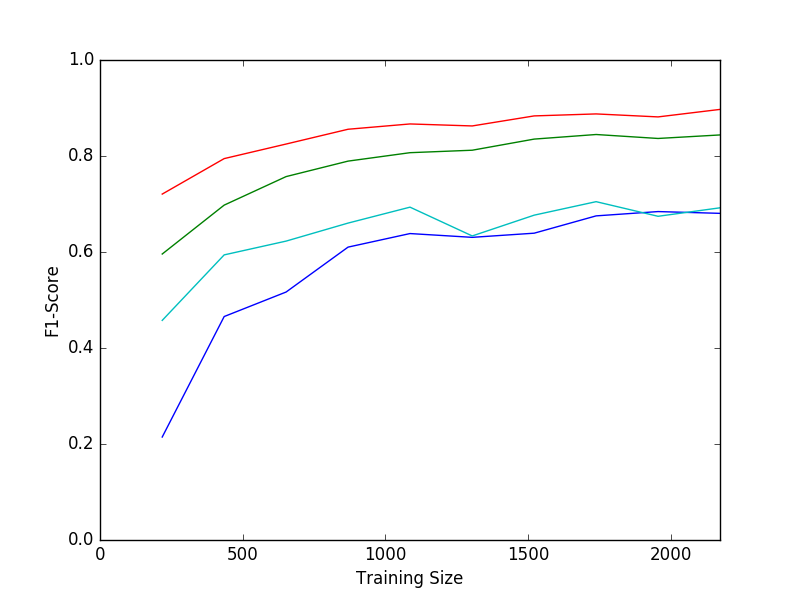
\includegraphics[width=16cm]{LR_comparison}
\textbf{Key:}

Blue is Naive Bayes

Green is Logistic Regression

Red is SVM

Teal is Random Forrest

\end{center}
\newpage

\subsection{Explanations}

For my experimentation SVM using a unigram model was the best performing classifier.  As a baseline I converted basic counts to frequencies using Term Frequency times Inverse Document Frequency to avoid the simple bag of words model.  SVM methods are particularly well suited for dealing with high dimensional features commonly found in text classification tasks.  Since text classification tasks tend to be linearly separable the strengths of SVM are fully utilized in this problem space.  The relatively poor performance of Naive Bayes, Logistic Regression and Random Forrest methods may be in part due to the nature of the training data since there were two distinct classifications regarding "Religion" in addition to the general advantages of SVM.

Regarding the learning rate results it is not surprising to find that as more training data is incorporated into the models the performance increases.  Perhaps the most interesting findings is how poorly Naive Bayes does given small training examples.  This may be due in part to the fact that with smaller training examples each feature has a stronger influence on the decision of the NB model.  Since NB uses a probabilistic model along with the Bayesian assumption there may be confusion induced in the model based on the occurrence of strings in documents which are not really related solely to the given document.  Only when given more training data does NB start to perform up to par with the other classification algorithms.
\\\\
\textbf{Sources:}\\
http://scikit-learn.org/stable/tutorial/text\_analytics/working\_with\_text\_data.html\\
https://www.cs.cornell.edu/people/tj/publications/joachims\_97b.pdf\\
http://blog.echen.me/2011/04/27/choosing-a-machine-learning-classifier/\\
http://www.nltk.org/book/ch06.html

\newpage
\section{My Best Configuration}
\subsection{Exploration Results}
All extensions used SVM as the classification algorithm.  I had trouble understanding the question prompt which is why there are more than 8 configurations included.

\begin{center}
 \begin{tabular}{||c c c c||} 
 \hline
 Configuration & Macro-Average F1 & Precision & Recall \\ [0.5ex] 
 \hline\hline
Removed Stopwords & 0.886653334361 & 0.92 & 0.91 \\
Porter Stemmed & 0.862612828581 & 0.90 & 0.89 \\ 
\textbf{Removed Stopwords + Porter Stemmed} & \textbf{0.890207820131} & \textbf{0.92} & \textbf{0.91} \\
Univariate Feature Selection  & 0.867678115483 & 0.90 & 0.90 \\ 
L2 Regularization & 0.860488785977 & 0.90 & 0.89 \\
L2 Regularization + Univariate Feature Selection  & 0.845426501587 & 0.89 & 0.88 \\ 
Univariate Feature Selection + L2 Regularization & 0.851530296806 & 0.89 & 0.89 \\
Removed Stopwords + Univariate Feature Selection & 0.886318523028 & 0.92 & 0.91 \\ 
 Removed Stopwords + L2 Regularization & 0.884554985184 & 0.92 & 0.91 \\
Porter Stemmed + Univariate Feature Selection & 0.857097005993 & 0.89 & 0.89 \\
Porter Stemmed + L2 Regularization & 0.862047021577 & 0.90 & 0.89 \\ 
* & 0.877267262495 & 0.91 & 0.90 \\ [1ex] 
 \hline
\end{tabular}
\end{center}

*Porter Stemmed + Removed Stopwords + Univariate Feature Selection

\newpage
\subsection{Explanations}
The strong performance of Porter stemming paired with removing stopwords seems to be a product of the strong effect that removing stopwords has on the overall accuracy of the model.  Since stopwords add so little the the classification problem (given that they occur in many contexts due to the nature of the language) removing them increases the classification power of the model.  To further enhance the models predictive power the use of Porter stemming translates sets of words into a common representation.  This gives a more accurate account of the relative frequencies of important features whereas without stemming there would be a more diluted representation as important words may have their frequencies spread between their slight variations.\\\\
\textbf{Sources:}\\
http://www.nltk.org/book/ch02.html\\
http://www.nltk.org/howto/stem.html\\
http://scikit-learn.org/stable/modules/feature\_selection.html\\
http://scikit-learn.org/stable/auto\_examples/feature\_selection/plot\_feature\_selection.html

\end{document}  